\part{系统架构与实现}

\begin{figure}[h]
\centering
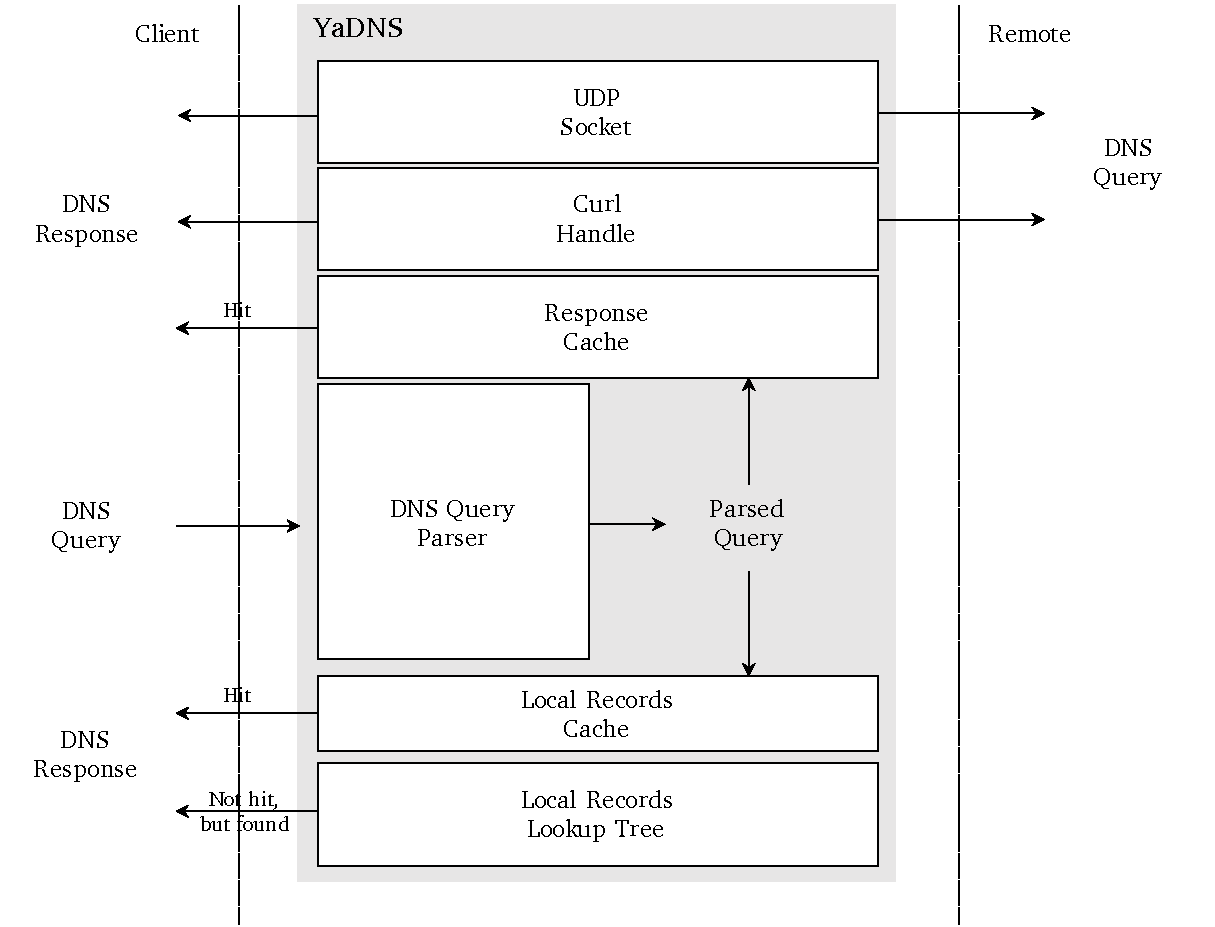
\includegraphics[width=0.8\textwidth]{figures/sys_arch}
\caption{YaDNS系统架构}
\label{fig:sys-arch}
\end{figure}

本节中将介绍YaDNS系统的整体架构与各个部分的具体实现。如图 \ref{fig:sys-arch} 中所示,YaDNS系统整体可以分为三个模块。第一个模块为DNS查询报文解析,负责将收到的DNS报文解析为具体的查询请求,用以后续对于是否命中本地记录的判断;第二个模块为本地记录的命中判断,YaDNS实现了一个高性能的LRU缓存,与一个多叉查找树。同时有一个缓存能够对远端服务器发来的资源进行缓存。若收到的查询请求为A型请求,则会检查请求的域名是否在本地记录中;第三个模块为DNS信息转发,若查询请求并非A型请求,或请求的域名不在本地记录中,则会将DNS报文转发给远端DNS服务器。转发的方式有两种:基于UDP套接字的普通DNS查询,与基于\lstinline{libcurl}发起HTTPS请求的DoH查询。除此以外,还有一些工具模块,如能够配置日志输出级别的日志模块,以及能够解析命令行参数的参数解析模块。接下来首先对系统的整体工作方式进行阐述,随后对各个部分的设计与实现分别进行描述。

\section{系统整体运行方式}

本节中首先提纲挈领地阐述YaDNS运行的主要方式,在运行过程中使用到的模块。随后对各个模块进行详细阐述。

程序开始运行后,首先调用参数解析模块对命令行参数进行解析,得到系统运行的配置,并进行相应的设置。随后初始化 \lstinline{libuv} 的事件循环,对程序使用到的各类资源进行初始化,调用本地记录模块加载本地记录信息,系统开始监听本地的53端口。

\begin{figure}[t]
  \centering
  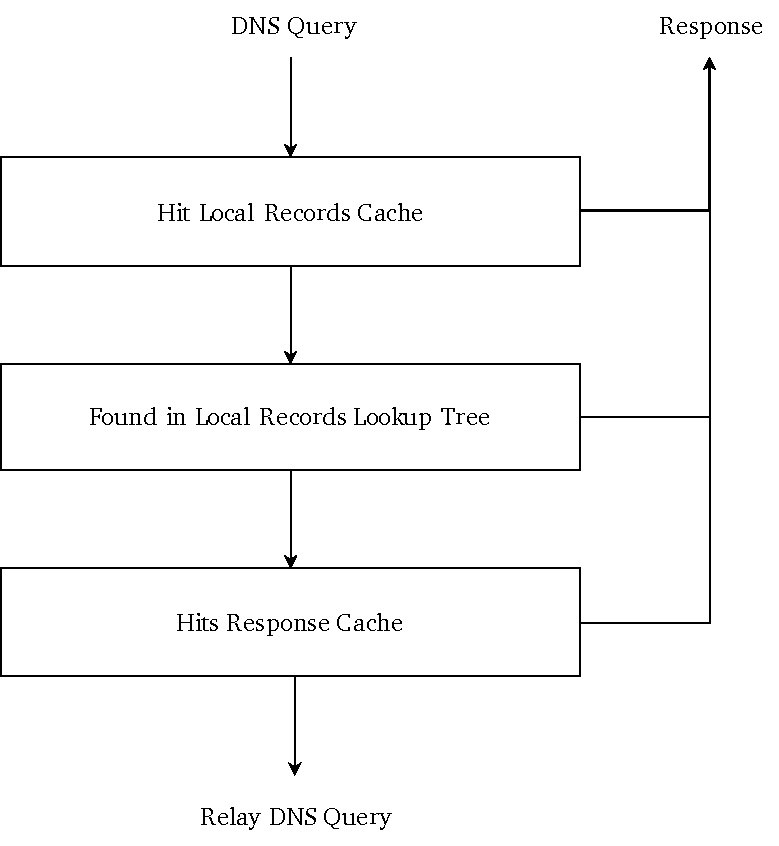
\includegraphics[width=0.5\textwidth]{figures/query}
  \caption{对收到的查询请求的处理}
  \label{fig:query}
\end{figure}

如图 \ref{fig:query} 中所示,当从53端口收到一个UDP报文时,首先调用DNS查询报文解析模块对报文进行解析,得到查询。若查询的问题是A类,则首先调用本地记录模块中的查询函数,查询请求的域名是否在本地记录中。若存在于本地记录中,则直接返回响应报文。若不存在,则再次调用本地记录模块中的查询函数,查询记录是否在响应缓存中,若有也直接返回。若仍然未找到,或查询的问题并非A类,则调用DNS转发模块对进行进行转发。这涉及到讲查询信息存入查询池中,并获得一个转发的句柄进行转发。

当YaDNS收到一个远端服务器发来的报文时,将会通过DNS编号(对于UDP转发而言)或连接上下文信息(对于DoH转发而言)获取与之对应的查询请求,并将其转发回客户端。除此以外,YaDNS也会解析收到的报文,对其中能够缓存的A类资源记录进行缓存。

\section{DNS查询报文解析}

DNS查询报文解析模块根据\href{https://tools.ietf.org/html/rfc1035}{RFC 1035}标准中规定的DNS信息格式对收到的DNS查询报文进行解析。解析的查询信息将被保存在如下的数据结构中。
\begin{lstlisting}[language=C]
struct dns_msg {
    char raw[DNS_MSG_MAX_LEN];
    uint32_t msg_len;
    dns_msg_header_t header;
    dns_msg_q_t question[DNS_MSG_MAX_ENTRY];
};
typedef struct dns_msg dns_msg_t;
\end{lstlisting}

可见,解析完成的报文中保存了原始信息、原始信息长度、报文头部信息、报文中问题节包含的DNS查询问题等。其中,解析的报文头部保存在如下的数据结构中。
\begin{lstlisting}[language=C]
struct dns_msg_header {
    uint16_t id;
    uint8_t qr;
    uint8_t opcode;
    uint8_t aa;
    uint8_t tc;
    uint8_t rd;
    uint8_t ra;
    uint8_t rcode;
    dns_size_t qd_cnt;
    dns_size_t an_cnt;
    dns_size_t ns_cnt;
    dns_size_t ar_cnt;
};
typedef struct dns_msg_header dns_msg_header_t;
\end{lstlisting}

而查询问题保存在下面的数据结构中:
\begin{lstlisting}[language=C]
struct dn_label {
    dns_size_t len;
    dns_size_t offset;
};
typedef struct dn_label dn_label_t;

struct dn_name {
    dn_label_t labels[DN_MAX_LABEL];
    dns_size_t len;
};
typedef struct dn_name dn_name_t;

struct dns_msg_q {
    dn_name_t name;
    uint16_t type;
    uint16_t class;
};
typedef struct dns_msg_q dns_msg_q_t;
\end{lstlisting}

注意到,由于解析的DNS请求的数据结构中包含了原始信息,为了节省空间,记录域名的每个标签时,只需要记录偏移量与长度即可。

DNS报文解析模块的实现严格遵守了RFC 1035标准中规定的各项要求。例如在RFC 1035标准中的第4.1.4节中提出的报文压缩策略也予以考虑实现。

包含了这一模块主要功能函数的头文件位于 \lstinline{include/dns/parse.h} 中。

\section{本地记录}

YaDNS能够加载本地域名记录。当请求的域名信息在本地记录中时,YaDNS不会进行转发,而是直接将本地记录返回。本地记录模块分为如下几个部分:记录文件的解析与加载、DNS响应报文的生成、LRU缓存、域名信息查找树。

\subsection{记录文件的解析与加载}

YaDNS能够加载文本格式的域名记录文件;每一行为一条记录,每条记录是以空格分隔的域名及其相应的IP地址。形式化地,
\begin{verbatim}
record ::= ip_addr ' ' domain_name
records ::= record | record '\n' records
\end{verbatim}

记录文件解析模块能够读取并解析记录文件中所有的域名记录信息。包含这一模块主要功能函数的头文件位于 \lstinline{include/db/io.h} 与 \lstinline{include/db/parse.h} 中。读取一个文件中的所有记录通过下面的函数完成。

\begin{lstlisting}[language=C]
dn_db_record_t *db_read_all_records(char *path, int *count, int *ret_code);
\end{lstlisting}

这一函数返回读取的记录列表头部指针,并且能够返回读取的记录数量与返回值。

\subsection{生成响应报文}

若在本地域名记录中查询到了请求的域名,则会生成响应报文返回给客户端。查询到的IP地址作为资源记录 \emph{(Resource Record)}放在报文的回答节中。生成的报文严格遵守RFC 1035中指定的报文格式。

\begin{figure}[t]
\centering
\begin{verbatim}
      +--+--+--+--+--+--+--+--+--+--+--+--+--+--+--+--+
      | 1  1|                OFFSET                   |
      +--+--+--+--+--+--+--+--+--+--+--+--+--+--+--+--+
\end{verbatim}
\caption{报文压缩中的域名指针格式}
\end{figure}

值得一提的是,在生成响应报文时,为了缩短报文长度,使用了RFC1035中第4.1.4小节提出的报文压缩 \emph{(Message Compression)} 策略。在返回报文中资源记录的域名部分,直接使用域名指针指向报文的问题节中查询域名的位置。

\subsection{域名记录的存储结构}

YaDNS使用多叉树来存储读取的域名记录。除此以外,YaDNS实现了一个LRU缓存,并且自行设计了适用于域名的哈希函数。缓存使用哈希函数进行直接映射,并且采用了两路组相联结构。

\subsubsection{多叉树}

\begin{figure}[h]
  \centering
  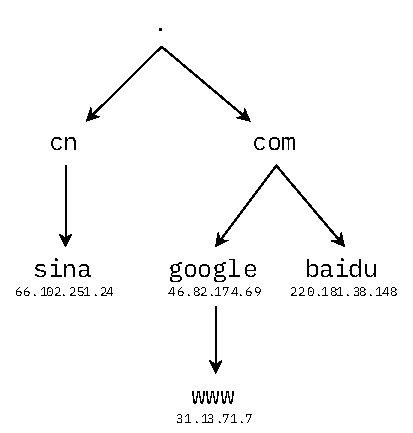
\includegraphics[width=0.5\textwidth]{figures/tree_example}
  \caption{域名记录多叉树例子}
  \label{fig:tree-example}
\end{figure}

存储域名记录信息的多叉树中,每个节点都包含域名中的一个标签。若某个节点存储了一条IP地址信息,则其对应的域名为从这一节点一直到根节点路径上所有标签的拼接。如图 \ref{fig:tree-example} 中所示的多叉树存储了表 \ref{tab:tree-example} 中所示的域名记录信息。

\begin{table}[t]
  \centering
  \begin{tabular}{cc}
  \toprule
  域名 & IP地址 \\
  \midrule
  sina.cn & 66.102.251.24 \\
  google.com & 46.82.174.69 \\
  www.google.com & 31.13.71.7 \\
  baidu.com & 220.101.38.148 \\
  \bottomrule
  \end{tabular}
  \caption{图 \ref{fig:tree-example} 中多叉树所存储的域名记录}
  \label{tab:tree-example}
\end{table}

下面形式化地给出域名信息多叉树的具体定义。为了方便表达,首先定义列表。
\begin{definition}[列表]
  对于某个集合$\mathcal X$,记$\mathds L(\mathcal X) = \bigcup_{i \ge 0} X^i$为包含集合$\mathcal X$中元素的列表。令$| \cdot | : \mathds I(\mathcal X) \rightarrow \mathds N$为长度函数。对于$l \in \mathds L(\mathcal X)$,用$l_{k} \in \mathcal X$表示列表中的第$k$个元素。记$\mathds L^k(\mathcal X) = \{ l \in \mathds L(\mathcal X) \mid | l | = k \}$为长度为$k$的列表。
\end{definition}

列表可以用来表示许多需要的数据结构。如域名可以表示为标签的列表,而多叉树的子孙节点也可以表示为一个列表。在实现中,列表可以用链表也可以用数组来表示。

\begin{definition}[域名记录多叉树]
  记$\mathcal I$为所有的IP地址,$\mathcal L$为所有的域名标签。则$\mathcal D \triangleq \mathds L(\mathcal L)$为所有的域名集合。定义多叉树的节点$\mathcal V \triangleq \mathcal L \times \mathcal I \cup \emptyset \mathcal \mathds L(\mathcal V)$。也即一个节点包含了一个标签、一个IP地址和一个子孙列表。特别的,根节点$R = \emptyset \cup \emptyset \cup V$。一棵多叉树可以用根节点来索引。
\end{definition}

\begin{algorithm}[h]
\caption{\textsc{TreeInsert}($v$, $d \in \mathcal D$, $p \in \mathcal I$)}
\label{algo:tree-insert}
\If{$|d| = 0$}{
  $v_{\text{ip}} \gets p$\;
}
\For {$u \in v_{\text{child}}$} {
  \If {$d_0 = u_{\text{label}}$} {
    \textsc{TreeInsert}($u$, $d_{1:}, p$)\;
    \Return\;
  }
}
$u \gets (d_0, \emptyset, \emptyset)$\;
\textsc{ListAppend($v_{\text{child}}, u$)}\;
\textsc{TreeInsert}($u$, $d_{1:}$, $p$)\;
\end{algorithm}

算法 \ref{algo:tree-insert} 为多叉树的插入算法。算法递归地将域名记录插入到多叉树中。其中\textsc{ListAppend}为列表插入算法。

\begin{algorithm}[h]
\caption{\textsc{TreeBuild}($r \in \mathds L(\mathcal D \mathcal I)$) $\rightarrow \mathcal V$}
\label{algo:tree-build}
$R \gets (\emptyset, \emptyset, \emptyset)$\;
\For {$(d, p) $ in $ r$} {
  \textsc{TreeInsert}($R$, $d$, $p$)\;
}
\Return $R$\;
\end{algorithm}

算法 \ref{algo:tree-build} 定义了多叉树的构造算法。算法首先构造一个空的根节点,随后一条条地将节点插入到多叉树中。

\begin{wrapfigure}{r}{0.57\textwidth}
\begin{minipage}{0.57\textwidth}
\begin{algorithm}[H]
\caption{\textsc{TreeLookup}($v \in \mathcal V$, $d \in \mathcal D$) $\rightarrow \mathcal I$}
\label{algo:tree-lookup}
\If {$|d| = 0$} {
  \Return $v_{\text{ip}}$\;
}
\For {$u$ in $v_{\text{child}}$} {
  \If {$u_{\text{label}} = d_0$} {
    \Return \textsc{TreeLookup}($u$, $d_{1:}$)\;
  }
}
\Return $\emptyset$\;
\end{algorithm}
\end{minipage}
\end{wrapfigure}

算法 \ref{algo:tree-lookup} 定义了对多叉树的查找算法。算法同样是递归定义的。若在多叉树中查找到域名,则返回对应的IP地址。若没有查找到域名,则会返回空。

\subsubsection{LRU缓存}

除了多叉查找树之外,YaDNS也设计并实现了一个LRU缓存。当需要查找域名时,首先在缓存中查找,若没有找到,再进入多叉树中查找,并且将多叉树中找到的信息存入缓存中。在缓存中查找域名所需的时间为$O(1)$。

YaDNS中的LRU缓存使用自设计的哈希函数进行直接映射,并且为多路相联,使用LRU策略进行换出。假设缓存参数为$S$行,路数为$W$。则缓存数据结构可以形式化地定义如下。

\begin{definition}[LRU缓存]
定义$\mathcal C = \mathds L^S (\mathds L^W(\mathcal D \times \mathcal I) \times \mathcal B)$。其中$\mathcal B$为LRU使用统计信息。
\end{definition}

具体地,缓存可以用如下伪代码来表示。

\begin{lstlisting}[language=C]
typedef CacheLine[S] LruCache;
typedef struct {
  CacheEntry entry[W];
  Bit lru;
} CacheLine;
typedef struct {
  DomainName domain;
  IP ip;
} CacheEntry;
\end{lstlisting}

注意,由于YaDNS中路数$W = 2$,因而\textbf{每一行的LRU统计信息只需要用一比特来表示即可。}这在下面会具体描述。

\paragraph{哈希函数设计}

LRU缓存使用一个哈希函数将每一条域名记录直接映射到缓存中的某一位置。假设缓存的行数为$S$为一个宽度为$w$的无符号整型变量可以表示的值的个数,也即$S = 2^w$。形式化地,我们需要一个函数$\theta : \mathcal D \rightarrow \{ 0, 1, \cdots, S - 1 \}$。为了获得这样的一个函数,假设已经有了一个标签的哈希函数$\gamma : \mathcal L \rightarrow \{ 0, 1, \cdots, S - 1 \}$,则可以定义$\theta$为
\begin{equation}
  \theta(d) = \square_{k=0}^{|d| - 1} \gamma(d_k),
\end{equation}
其中$\square$为可选的二元运算符。在YaDNS使用的缓存中为$\oplus$也即异或运算符。

接下来考虑对于标签也即一个字符串的哈希函数。有许多经典而广发的字符串哈希函数,在YaDNS中使用了
\begin{equation}
  \gamma(l) = \sum_{i=0}^{|l| - 1} l_i \cdot p^i,
\end{equation}
其中因子$p$在实现中选择为$31$。

YaDNS使用的哈希函数实现了高效的域名映射。当$S = 256$也即缓存总大小为512行时,在给出的示例记录文件的909条记录中,缓存的利用率为$91.8\%$。
%附录 \ref{sec:hash-func-benchmark} 中包含了对哈希函数的详细测试。

\paragraph{LRU换出策略的实现}

LRU (Least Recently Used)是一种广泛使用的缓存换出策略。无论是在硬件还是软件缓存中,LRU都可以被用来决定在换出发生时需要换出的行。LRU需要统计\textbf{最近最少使用的路}来决定换出选择。具体地,LRU策略需要维护一个队列。假设某一缓存共有$N$路,分别记为$0, 1, \cdots, N-1$。则LRU需要保存一个装有所有路的标号的队列,当第$k$路被访问时,若当前队列状态为
\begin{equation}
q_1, q_2, \cdots, q_{a-1}, k, q_{a+1}, \cdots, q_{N-1},
\end{equation}
则将队列更新为
\begin{equation}
q_1, q_2, \cdots, q_{a-1}, q_{a+1}, \cdots, q_{N-1}, k.
\end{equation}

当换出发生时,直接从队列首部弹出一个标号即为选择换出的路。并将这个标号装入队尾。

YaDNS中的缓存实现为两路,因而对于每一行,只需要一个比特位就能够完成对LRU统计信息的记录,确定需要换出哪一行。具体地,若将两路分别标号为0与1。则相应的队列状态仅有两种:$0, 1$与$1, 0$。

\begin{figure}[h]
  \centering
  \begin{tikzpicture}[node distance=3cm,on grid,auto] 
    \node[state,initial] (q_01) {$0,1$}; 
    \node[state] (q_10) [right=of q_01] {$1,0$};
    \path[->] 
      (q_01) edge [bend left] node {visit 0} (q_10)
             edge [loop above] node {visit 1} ()
      (q_10) edge [bend left] node {visit 1} (q_01)
             edge [loop above] node {visit 0} ();
  \end{tikzpicture}
  \caption{LRU队列抽象成的自动机}
  \label{fig:lru-automata}
\end{figure}

LRU队列可以被抽象为图 \ref{fig:lru-automata} 中的有限状态自动机。由于只有两种状态,因而使用1比特就能够表示。根据对缓存的访问情况更新状态,即能够通过LRU策略选取换出行。

\subsubsection{时间与空间性能分析}
\label{sec:time-space-complexity}

接下来,对多叉树和缓存的效率进行分析。

\paragraph{多叉树的查找效率}

为了对多叉树的效率进行分析,假设域名的最大长度为$K$,而域名每一级可能的标签集合分别为$\mathcal L_1, \mathcal L_2, \cdots, \mathcal L_K$。假设查找的域名$d$在多叉树内,域名的每一级的标签$d_i \in \mathcal L_i, i = 1, 2, \cdots, K$,且每一级的标签服从两两独立的分布,$d_i \sim p_i$且$\forall j, p(d_i | d_j) = p(d_i)$,则查找时间的期望
\begin{equation}
  \mathds E [T] = \sum_{i = 1}^K \sum_{d_i \in \mathcal L_i} p_i(d_i) \tau |\mathcal L_i|,
\end{equation}

其中$\tau | L_i |$为在一个大小为$| L_i |$,随机排列的列表中线性查找一个元素所需的平均时间。这里的分布$p_i$在大多数时候是一个长尾分布。

因而,
\begin{equation}
\begin{split}
  \mathds E[T] &= \sum_{i=1}^K \tau | \mathcal L_i | \sum_{d_i \in \mathcal L_i} p_i(d_i) \\
  &= \sum_{i=1}^K \tau | \mathcal L_i |,
\end{split}
\end{equation}
也即多叉树的查找时间约为$O(\sum_{i=1}^K | \mathcal L_i |) \approx O(KN)$,其中$N$为每一级标签个数的平均值。

作为比较,若直接在一张线性表中查找域名信息,则需要的时间期望约为
\begin{equation}
  \mathds E[T^\prime] = \tau \prod_{i = 1}^K | L_i |,
\end{equation}
也即查找时间约为$O(\prod_{i=1}^K | \mathcal L_i |) \approx O(N^K)$。

\paragraph{缓存的查找效率}

由于采用了哈希函数直接映射的方式,缓存的查找效率近似于常数时间。需要的时间大多用于计算哈希函数值。而计算哈希函数的时间只与标签长度和域名级数有关,这两个值都可以被认为是常量。

\paragraph{LRU状态转移法的推广与效率分析}

对于一个有$N$路的缓存,最朴素的方法是为其显式地维护一个队列,根据访问情况更新队列,在需要换出是直接读取队首。而YaDNS中使用比特来表示LRU信息,本质上是一种查表法。推广来说,对于一个有$N$路的缓存,其访问状态共有$N!$种情况。则需要$\lceil \log_2 N! \rceil$位比特来存储状态。为其构建一张查找表,则需要$N! \lceil \log_2 N! \rceil \in O(N! \log_2 N!)$的空间。由Stirling近似,可知这个值近似于$O(N! \cdot N \log N)$。而若简单地维护一个队列,其空间复杂度仅仅位$O(N \log N)$。因而这样的查表法并不适用于$N$很大时,而在$N$很小时,查表法才能使用近乎等同的空间实现更快的返回速度(如当$N = 2$时,也即YaDNS的缓存中使用的路大小)。

\subsection{响应缓存的设计与实现}

YaDNS实现了一个基于 \lstinline{Trie} 的响应缓存来缓存从远端服务器收到的响应中的A类资源记录。在下面一段时间内,若再次查询缓存的域名,则可以直接返回,无需从远端服务器再次查询信息,加快了对频繁热点数据的返回时间,减少了带宽占用,提升系统整体效率。

首先,给出 \lstinline{Trie} 树的定义。首先给出 \lstinline{Trie} 树节点的定义。

\begin{definition}[Trie树节点]
  定义 $\mathcal C$ 为所有字符的集合。则对于任意一个集合$\mathcal X$,可以定义$\mathcal T \triangleq \mathcal C \times \mathds L(\mathcal T) \times \mathcal X$。注意这是一个递归定义,一个最基本的 Trie 树节点可以写为$r = (\emptyset, \emptyset, \emptyset)$,这一般可以作为初始化一棵Trie树时的根节点。
\end{definition}

可见,一个 \lstinline{Trie} 树的节点包含了这个节点所存储的字符、它的子孙节点的列表以及它存储的值。在定义了 \lstinline{Trie} 树的节点之后,就能够用一个根节点来索引一棵 \lstinline{Trie} 树,一般地,一棵 \lstinline{Trie} 树可以写为 $t = (\emptyset, \mathbf L, \emptyset)$,其中$\mathbf L$为根节点的子孙节点的列表。注意根节点的字符一般定义为空字符,且在根节点上不存储数据。

\lstinline{Trie} 树可以用伪代码表达如下。
\begin{lstlisting}[language=C]
typedef struct {
  Char key;
  X value;
  List[TrieNode] children;
} TrieNode[X];
\end{lstlisting}
其中\lstinline{X}为需要存储的值的类型。

接下来定义 \lstinline{Trie} 树的插入和查找算法。

\begin{algorithm}[h]
\caption{\textsc{TrieInsert}($r$, $s \in \mathds L(\mathcal C)$, $x \in \mathcal X$)}
\label{algo:trie-insert}
\textsc{ASSERT}($r$)\;
\If {$s$ is empty} {
  $r$.value $\gets x$\;
  \Return\;
}
\For {$c \in r$.children} {
  \If {$c$.key $= s_0$} {
    \textsc{TrieInsert}($c$, $s_{1:}$, $x$)\;
    \Return\;
  }
}
$u \gets (s_0, \emptyset, \emptyset)$\;
\textsc{ListAppend}($r$.children, $u$)\;
\textsc{TrieInsert}($u$, $s_{1:}$, x)\;
\end{algorithm}

\begin{algorithm}[h]
\caption{\textsc{TrieLookup}($r$, $s \in \mathds L(\mathcal C)$)}
\label{algo:trie-lookup}
\If {$r$ is empty} {
  \Return $\emptyset$\;
}
\If {$s$ is empty} {
  \Return $r$.value\;
}
\For {$c \in r$.children} {
  \If {$c$.key $= s_0$} {
    \Return \textsc{TrieLookup}($c$, $s_{1:}$)\;
  }
}
\end{algorithm}

在获得了算法 \ref{algo:trie-insert} 和算法 \ref{algo:trie-lookup} 中定义的 \lstinline{Trie} 树插入与查找算法之后,可以很容易地设计出一个能够缓存域名与IP地址的缓存。对于报文中的域名,直接使用 \lstinline{.} 分隔的字符串作为其索引,IP作为数据,插入一棵 \lstinline{Trie} 树中即可。

然而,还需要考虑记录失效与记录的删除问题。对记录失效的判断与删除的操作是惰性的 \emph{(lazy)},这意味着只有在查找到某条记录的时候,才会判断其是否失效,若失效,则删除。而不是隔一段时间就清理到期的记录。

对记录的清理是很容易的,直接将对应节点存储的数据赋值为空即可。然而,还有一个问题需要解决:在删除记录之后,\lstinline{Trie} 树中将存在许多的无用节点。他们在原先节点的路径上,却不存储数据。若缓存的某条记录在此后一直没有再次被访问,这些节点将一直处于无用状态,浪费内存。因而,需要设计对于\lstinline{Trie}树的垃圾回收算法。

\begin{algorithm}[h]
\caption{\textsc{TrieCleanup}($r$) $\rightarrow \{ 0, 1 \}$}
\label{algo:trie-cleanup}
\If {$r$ is empty} {
  \Return $1$\;
}
$n \gets 0$\;
$l \gets \emptyset$\;
\For {$c \in r$.children} {
  \If {\textsc{TrieCleanup}($c$) $= 0$} {
    $n \gets n + 1$\;
    \textsc{ListAppend}($l$, $c$)\;
  }
}
$r$.children $\gets l$\;
\If {$n = 0$} {
  \textsc{TrieDeinit}($r$)\;
  \Return 1\;
}
\Return 0\;
\end{algorithm}
其中,\textsc{TrieDeinit}能够释放\lstinline{Trie}占用的资源。上面的算法实现了对 \lstinline{Trie}树的垃圾回收。在得到上面的所有算法之后,我们就能使用\lstinline{Trie}树很好地管理缓存的资源记录了。

\section{DNS请求转发}

\begin{figure}[h]
  \centering
  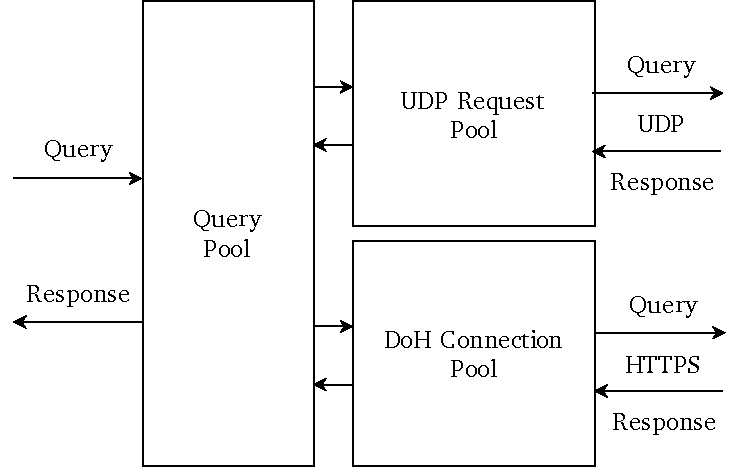
\includegraphics[width=0.7\textwidth]{figures/relay}
  \caption{消息转发系统模块图}
  \label{fig:relay}
\end{figure}

当YaDNS收到的请求无法在本地记录中找到时,将会转发到远程服务器。YaDNS支持两种不同的转发方式:简单UDP转发与DoH转发。

具体地,如图 \ref{fig:relay} 中所示,当有一个需要转发的DNS请求报文时,首先将其存入查询池 \emph{(Query Pool)} 中。然后,根据程序设置,选择从UDP池 \emph{(UDP Pool)} 或DoH连接池 \emph{(DoH Connection Pool)} 中获取一个传输句柄来与远端服务器进行通信。下面分别介绍UDP与DoH转发的具体实现。

\subsection{UDP转发}

UDP转发使用\lstinline{libuv}提供的UDP接口来向远端服务器发送UDP报文。UDP转发使用同一个套接字发送所有需要发送的UDP报文,并通过对DNS编号的处理来分辨不同客户端发来的请求与对应的响应。

具体地,当获得一个需要转发的DNS查询时,首先存入查询池,并从UDP池获取一个句柄。句柄保存的上下文数据结构定义如下。

\begin{lstlisting}[language=C]
typedef struct {
    int query_id;
    int dns_id;
    char send_buf[UDP_CONTEXT_BUF_SIZE];
    size_t send_len;
    char valid;
    void *timer;
} udp_context_t;
\end{lstlisting}

可见,句柄保存了与其绑定的查询在查询池中的编号。且会将DNS信息复制一份,以方便对DNS报文编号的修改。它也包含了一个 \lstinline{valid} 域来指示这个句柄是否处于使用状态,以及一个 \lstinline{timer} 域包含一个指向 \lstinline{libuv} 的 \lstinline{timer} 句柄的指针。这个timer会管理请求的超时。

而UDP池数据结构的定义如下:

\begin{lstlisting}[language=C]
typedef struct {
    udp_context_t **pool;
    size_t pool_size;
    queue_t *idx_queue;
    uint16_t next_dns_id;
} udp_pool_t;
\end{lstlisting}

可见,UDP池保存了UDP句柄的列表,存储了池子的大小,也包含一个队列。队列中存储了池子中空闲的编号,在初始化时,将会将池子中所有的编号按需存入队列中。当需要分配一个新的UDP句柄时,则从这一队列中取出编号,当有一个UDP句柄空闲时,则将相应的编号存回队列中。

\paragraph{DNS编号的分配与处理} 除此以外,UDP池还维护了一个变量来保存为下一个请求分配的DNS编号。当分配新的UDP句柄时,将当前保存的编号分配给这个请求,并且将 \lstinline{next_dns_id} 递增。在初始化时,这个值被初始化为当前时间。

由于YaDNS通过同一个UDP套接字转发所有的请求,因而为每一个转发的请求分配不同的DNS编号,而不是直接使用客户端发来的报文中使用的编号是必须的。若客户端A与B几乎同时发来了一个DNS查询报文,其编号刚好都为$x$。若直接将报文转发,而不对其中的DNS编号进行处理,则在收到远端服务器返回的响应时,无法分辨两个编号为$x$的响应报文究竟属于哪个客户端。从而导致错误。

因而在YaDNS中,会将转发的DNS报文中的编号修改为分配给相应UDP句柄的编号。由于保证分配给UDP具柄的编号在绝大多数时候是独立的,可以将相应的编号唯一地与一个UDP上下文绑定,也就可以确定响应报文所对应的客户端。在找到对应的客户端后,将报文中的编号改为原始编号,即可以转发给客户端。

\paragraph{UDP超时}

由于UDP提供的是\textbf{不可靠的传输服务},因而可能会出现数据包丢失的情况。因而为UDP请求设置超时时间是必要的。一方面,若发生丢包,没有超时机制的请求将一直被挂起,占用资源。另一方面,超时机制也能够保证DNS编号不会发生重复。考虑一个YaDNS服务器以$p$个每秒的速度收到客户端发来的查询请求,DNS编号的宽度$w=16$,因而有$2^w$个不同的编号。在$\frac {2^w} p = \frac {65536} p$秒后,分配的DNS编号就会发生重复。需要指出,在大多数情况下,因为UDP报文的传输速度缓慢而造成编号重复、混淆是不可能发生的。UDP报文的来回时间一般不会超过$8$秒,在$8$秒内出现两个相同编号的报文则需要$p = 8192$。在这样的较高负载场景下,基本不可能使用单台机器的单个套接字与远端服务器通信。尽管如此,这种情况还是需要在设计时予以考虑。

\subsection{DoH转发}

DOH转发的本质是进行HTTPS请求。YaDNS在实现中使用 \lstinline{libcurl} 的 Multi 接口,结合 \lstinline{libuv} 进行非阻塞的并发HTTPS请求。

DoH转发同样有连接池的设计。连接池的数据结构定义如下。

\begin{lstlisting}[language=C]
typedef struct {
    CURL *easy_handle;
    int query_id; // associated query id
    char read_buf[CONN_CONTEXT_BUF_SIZE];
    char send_buf[CONN_CONTEXT_BUF_SIZE];
    size_t send_len;
    size_t nread;
    uint16_t dns_id;
    int conn_id;
    void *timeout_timer;
} conn_context_t;
\end{lstlisting}

可见,连接池中的连接句柄共保存了下面这些上下文字段:
\begin{enumerate}
  \item \lstinline{libcurl}连接句柄;
  \item 与连接绑定的查询在查询池中的编号;
  \item 从服务器接收的缓冲区;
  \item 发送缓冲区;
  \item 分配的DNS编号;
  \item 连接编号;
  \item 超时定时器的句柄。
\end{enumerate}

DoH连接池的设计与DoH转发的实现与UDP转发是类似的。一个区别在于DoH连接使用了 \lstinline{Curl} 提供的HTTPS请求句柄来发送和接收DNS报文。除此以外,需要指出在DoH连接中,重新分配DNS编号不是必要的。原因在于不同的DNS查询使用不同的 \lstinline{Curl}句柄完成,而一个\lstinline{Curl}句柄完成的DNS查询在一次HTTPS传输中独立完成,并不存在混淆的情况。而每个\lstinline{Curl}句柄也通过连接上下文唯一地与一个客户端请求绑定。然而,为了保持与UDP转发在实现上的一致性,DoH转发同样实现了对DNS编号的分配与处理。

注意,通过连接池的实现,YaDNS实现了对\lstinline{Curl}句柄的复用。这一方面更好地利用了资源,免去了每次转发都需要初始化再销毁\lstinline{Curl}句柄的繁琐,另一方面,复用\lstinline{Curl}也意味着复用了TCP连接。在短时间频繁转发请求的情况下,复用HTTPS连接 \emph{(Keep Alive)} 能够省去TCP、TLS握手的环节,大幅提升响应速度。

\section{工具模块}

本节将介绍YaDNS的工具模块:日志输出与命令行参数解析。

\begin{figure}[h]
  \centering
  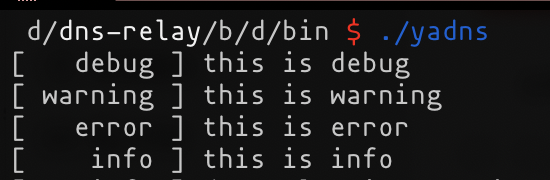
\includegraphics[width=0.6\textwidth]{figures/logging}
  \caption{日志输出模块示例}
  \label{fig:logging}
\end{figure}

\subsection{日志输出}

YaDNS实现了简单的日志分级输出功能,共分为4级:调试信息、警告信息、错误信息、用户信息。对应了四个日志函数:\lstinline{logd}, \lstinline{logw}, \lstinline{loge}, \lstinline{logi}。通过模块提供的 \lstinline{logging_init} 函数,能够对输出等级进行设置。
\begin{lstlisting}[language=C]
void logging_init(char level);
\end{lstlisting}
其中\lstinline{level}为等级掩码,有且仅有低4位比特有效。4位比特从高到低分别对应调试信息、警告信息、错误信息、用户信息,当对应比特为1时,输出信息,为0时,不输出信息。如图 \ref{fig:logging} 中给出了日志输出模块的运行示例。

\subsection{命令行参数解析}

YaDNS实现了一个简单的命令行参数解析模块,能够解析命令行参数进行系统配置。参数解析模块的接口设计参考了\textbf{Python的\lstinline{argparse}模块}。参数解析模块支持很多不同类型的参数。如下给出的函数调用添加了一个参数,其标示为\lstinline{server},类型为字符串。并且给出了描述和默认值。
\begin{lstlisting}[language=C]
ap_add_argument(ap, "server", AP_STR, "Raw remote DNS server address (default 114.114.114.114).", "114.114.114.114");
\end{lstlisting}
在这样设置之后,就可以这样运行程序:
\begin{verbatim}
./yadns --server your.udp.dns.server
\end{verbatim}
在Python的\lstinline{argparse}模块中,相应的调用为
\begin{lstlisting}[language=Python]
parser.add_argument('--server', type=str, help='Raw remote DNS server address (default 114.114.114.114).', default='114.114.114.114')
\end{lstlisting}

下面的例子设置了一个类型为开关的参数:
\begin{lstlisting}[language=C]
ap_add_argument(ap, "doh_proxy", AP_STORE_TRUE, "Enable DoH proxy mode.", 0);
\end{lstlisting}
添加的参数标示为\lstinline{doh_proxy},给出了描述,没有默认值。对于开关类参数而言,默认值即为0。可以如下面这样运行程序:
\begin{verbatim}
./yadns --doh_proxy
\end{verbatim}
这样将会设置这个开关。

同时,命令行参数解析模块也能根据给出的描述信息,自动输出帮助信息。当系统运行时只提供了开关 \lstinline{--help} 时,将打印出帮助信息。下面给出了运行时输出的例子。
\begin{verbatim}
$ ./yadns --help
dns-relay -- Simple dns proxy, with DoH
  --help
    Display this helper text.
  --server STR
    Raw remote DNS server address (default 114.114.114.114).
  --doh_server STR
    Remote DoH server address (default cloudflare-dns.com).
  --doh_proxy
    Enable DoH proxy mode.
  --max_query INT
    Max concurrent query number (default 32).
  --max_doh_conn INT
    Max concurrent DoH connection number (default 32).
  --max_udp_req INT
    Max concurrent UDP request number (default 32).
  --curl_verbose
    Enable verbose curl debug output.
  --client_port INT
    Client UDP socket port for raw DNS request (default 2345).
  --hosts_path STR
    Path to hosts file.
  --logging INT
    Logging mask for controlling output verbosity (default 15).
\end{verbatim}
















